\documentclass{beamer}
\usepackage{graphicx}
\usepackage{tikz}
\usetikzlibrary{shapes,arrows}
\usepackage{tikz}
\usepackage{}
\usetheme{default}
%\usecolortheme{seahorse}
\usepackage{default}

  \setbeamertemplate{footline}[page number]
\setbeamertemplate{navigation symbols}{}
\setbeamertemplate{frametitle}[default][center]
\setbeamerfont{frametitle}{shape=\scshape}

\usepackage{color}

{\title{\textsc{Applying Simple Intertemporal Economics to Covid-19}}
\author{Trevor S. Gallen}
\date{}



\begin{document}


\begin{frame}
\titlepage
\end{frame}

\begin{frame}
\frametitle[alignment=center]{Introduction}
\begin{itemize}
\item What use is intertemporal thinking?
\bigskip
\item Simple but important application: how willing should we be to trade off lives for economic harm in COVID-19 pandemic?
\bigskip
\item If only killed 500,000 terminally-ill people with a few minutes left to live, probably not worth \$3 trillion for 60 minutes more each (\$100,000/life-minute).  
\bigskip
\item But if save lives of 500,000 people who would otherwise live for 60 more years, potentially worth it (\$0.19 per life-minute saved)
\bigskip
\item IVT-type argument:  there's a place where we're indifferent!
\bigskip
\item Worth stopping here: do you agree?  Because many politicians and some economists claim not to agree.
\end{itemize}
\end{frame}

\begin{frame}
\frametitle[alignment=center]{Hall, Jones, and Klenow (2020)}
\begin{itemize}
\item Enter Hall, Jones, and Klenow (2020)
\bigskip
\item How do we think about that tradeoff?
\bigskip 
\item Write down a simple model of people consuming and risking death.  So, value $V$ of living at some age $a$ is, given probability of given age $a$ at time $t$ of $S(a,t)$:
$$\textcolor{red}{V_a}=\textcolor{blue}{\sum_{t=0}^\infty}\textcolor{green}{\beta^t}\textcolor{orange}{S(a,t)}\textcolor{gray}{u(c_t)}$$
\begin{itemize}
\item $\textcolor{red}{V_a}$: value of being alive at age a
\item $\textcolor{blue}{\sum_{t=0}^\infty}$: sum over all future periods
\item $\textcolor{green}{\beta^t}$: discount the future
\item $\textcolor{orange}{S(a,t)}$: only value if you survive
\item $\textcolor{gray}{u(c_t)}$: get utility from consumption/being alive
\end{itemize}
\item Do you disagree? If so, let us know in discussion forum!
\end{itemize}
\end{frame}

\begin{frame}
\frametitle[alignment=center]{Value of being alive}
\begin{itemize}
\item Value of being alive at age $a$ is:
$$V_a=\sum_{t=0}^\infty\beta^tS(a,t)u(c_t)$$
\item Can rewrite this as
$$V_a=u(c_0)+\beta S(a,1)V_{a+1}$$
\item In other words, value of being alive at age $a$ is initial utility plus discounted ($\beta$) value of waking ($V_{a+1}$) up tomorrow, times probability you actually wake up ($S(a,1)$)
\end{itemize}
\end{frame}

\begin{frame}
\frametitle[alignment=center]{Social Planner (Politician's) Problem}
\begin{itemize}
\item What is trade off problem for benevolent social planner/politician?  
\bigskip
\item Need to know populations: $N$ is number of people (normalize old population to 1)
\bigskip
\item COVID-19 reduces survival rate of old to $S-\delta$ for one period
\bigskip
\item What is tradeoff between reduction in consumption $\lambda$ and $\delta$? (denote young $y$ and old $o$)
\bigskip
$$W(\lambda,\delta)=(N-1)V_y+1\cdot V_0$$
\item Utilitarian treating people equally here
\end{itemize}
\end{frame}

\begin{frame}
\frametitle[alignment=center]{Maximizing Welfare}
\begin{itemize}
\item The social planner wants to choose consumption drop $\lambda$ and death rate reduction$\delta$ to maximize utility:
\begin{align*}
W(\lambda,\delta) & =(N-1)V_y+1\cdot V_0\\
 & = (N-1)\left[u(\lambda c_0)+\beta S_yV(F,y)\right]+\left[u(\lambda c_0)+\beta(S_0-\delta)V_{F,o}\right]
 & =  Nu(\lambda c_0)+(N-1)\beta S_yV_{F,y}+\beta(S_0-\delta)V_{F,o}
\end{align*}
\item Where $V_F$ is utility if survive
\item $W(\lambda,0)$ is welfare when death rate is zero (but consumption reduced by some amount)
\item $W(1,\delta)$ is welfare when consumption does not decline but death rate is untouched (baseline)
\item How much are we willing to pay to reduce death rate to zero?  $\lambda$ that solves this problem tells us: $W(\lambda,0)=W(1,\delta)$
\end{itemize}
\end{frame}

\begin{frame}
\frametitle[alignment=center]{Skipping Math}
\begin{itemize}
\item The authors take the equation, take a Taylor expansion of utility around no drop in consumption (linearize utility functions(\textcolor{red}{!})) and plug into our problem to find the tradeoff:
$$1-\lambda=\frac{\beta\delta}{N}\frac{V_{F,o}}{u'(c_0)c_0}$$
\item Letting $\alpha=1-\lambda$ be the amount you'd give up to solve the crisis completely, and letting $LE$ be life expectancy of old:
\item Also let $v=u(c)/(u'(c)c)$ be value of one more year of life relative to consumption (convert consumption to life-years)
$$\textcolor{red}{\alpha}=\frac{\textcolor{blue}{\delta}\textcolor{green}{v}\textcolor{orange}{LE_o}}{\textcolor{cyan}{N}}$$
\item \textcolor{red}{$\alpha$}: Pay in fraction of consumption drop
\item \textcolor{blue}{$\delta$}: Pay more when death rate higher
\item \textcolor{green}{$v$}: Pay more when life more than consumption
\item \textcolor{orange}{$LE_o$}: Pay more when old have long life ahead of them
\item \textcolor{cyan}{$N$}: Pay less when they are a smaller fraction of population
\end{itemize}
\end{frame}

\begin{frame}
\frametitle[alignment=center]{Calibrate the Model}
\begin{itemize}
\item The following are the author's best-guesses from the literature:
\begin{itemize}
\item Death rate of 0.81\% without mitigation efforts $\delta=0.0081$
\item Consumption represents 1/3 of happiness in life $v=3$
\item Life expectancy $LE_o=14.47$ years
\item $N=1$ (first assume everyone is facing the same mortality risk)
\end{itemize}
\item From these, get $\alpha=0.35$!  Willing to pay 35\% of consumption to solve crisis.
\end{itemize}
\end{frame}

\begin{frame}
\frametitle[alignment=center]{Robustness}
\begin{figure}
\centering
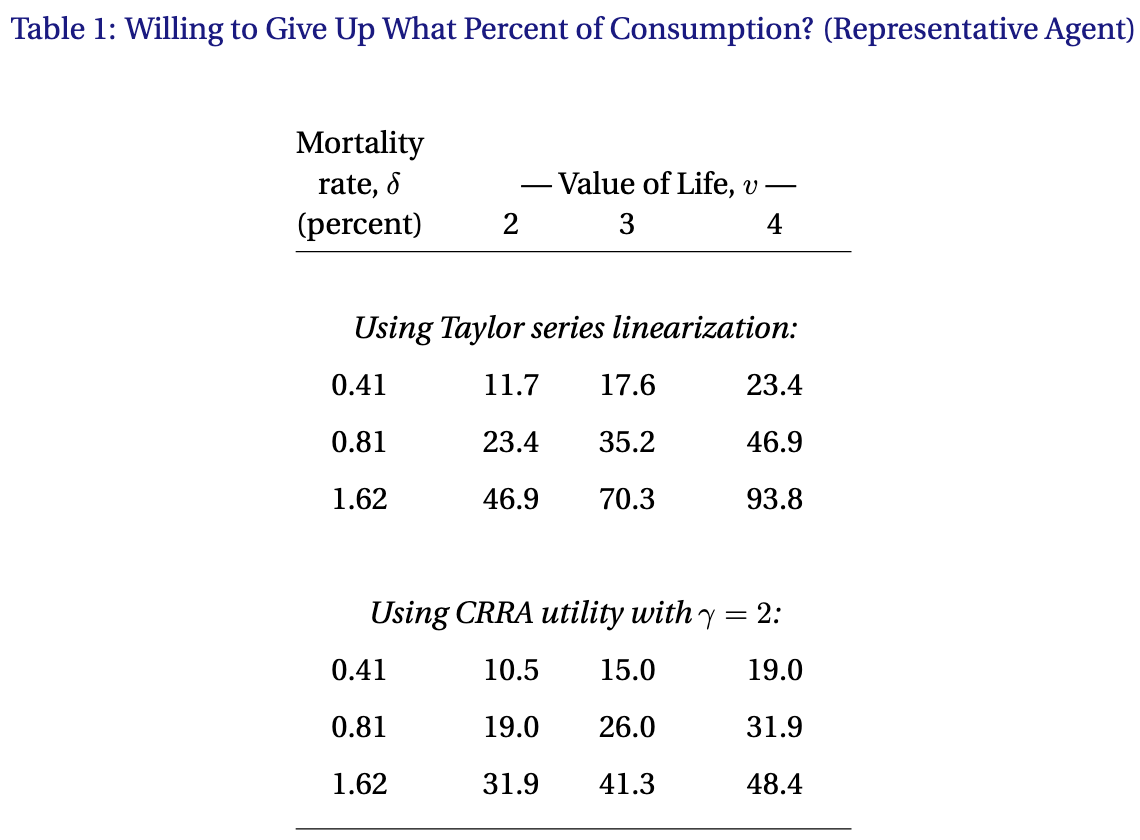
\includegraphics[scale=0.5]{Halletal_2020.png}
\end{figure}
\end{frame}

\begin{frame}
\frametitle[alignment=center]{Calibrate the Model}
\begin{itemize}
\item Assumption that everyone is young is dumb!
\begin{itemize}
\item Death rate of 3.86\% without mitigation efforts for old, including virus contraction rate without mitigation of 75\% (is this a good assumption?)
\item Life expectancy shorter:  $LE_o=10.9$
\end{itemize}
\item From these, get $\alpha=0.21$!  Willing to pay 21\% of consumption to solve crisis.
\bigskip
\item Note that if current mitigation only drops 50\%, willing to pay only 10.5\% drop
\end{itemize}
\end{frame}

\begin{frame}
\frametitle[alignment=center]{Robustness}
\begin{figure}
\centering
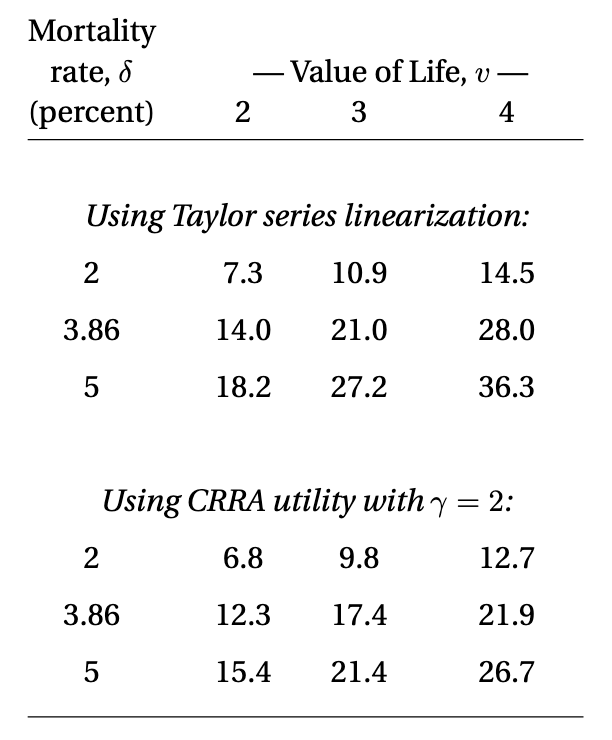
\includegraphics[scale=0.5]{Halletal2_2020.png}
\end{figure}
\end{frame}

\begin{frame}
\frametitle[alignment=center]{Iconoclastic Calibration}
\begin{itemize}
\item Death rate of older of 5.15\%, but let's say due to asymptomatic/non-reporting of those who don't have complications it's really 70\% that.  Assume older mitigation is 60\% getting it 
\item But drop in death rate is only half (we aren't perfect):  $\delta=0.0515*0.7*0.6*0.5=0.0108$
\item For ``realistic" mitigation efforts, should only be willing to pay:
$$\alpha=\frac{0.0108\cdot 3\cdot 10.9}{5}=7.06\%$$
\item 
\end{itemize}
\end{frame}

\begin{frame}
\frametitle[alignment=center]{Comparing other Estimates}
\begin{itemize}
\item These give willingness to pay of between \$1.3 trillion and \$6 trillion
\bigskip
\item Luigi Zingales: \$9 million per lost life above 65, 7.2 million deaths prevented, \$65 trillion
\bigskip
\item Why so different?  Way higher (6x) on value of life and death rate (4.5x) (9 million baseline deaths compared to 2 million in Hall, Jones, and Klenow)
\bigskip
\item Fortunately these are empirical questions
\end{itemize}
\end{frame}



\begin{frame}
\frametitle[alignment=center]{Conclusions/Discussion}
\begin{itemize}
\item People make tradeoffs between life expectancy and consumption all the time
\smallskip
\item Crazy (welfare-decreasing) to make dramatically different decisions than they would make
\smallskip
\item People are willing to trade of life-minutes for own consumption (and consumption of their children)
\smallskip
 \item My own conclusions: \textbf{on utilitarian grounds} honest people can disagree whether or not a decline between 7\% and 30\% of consumption is a reasonable cost to pay, depending on how effective mitigation and on facts
 \smallskip
 \item Outside those bounds, probably making the average person worse off (but maybe you have moral reasons, or a calibration like Zingales's)
 \smallskip
  \item Benefit of economic thinking: you don't have to call people ghouls or death eaters when they disagree--just correct their calibration or model!
\end{itemize}
\end{frame}

\end{document}